\documentclass{beamer}

\usepackage[french]{babel}
\usepackage[T1]{fontenc}
\usepackage[export]{adjustbox}
\usepackage{graphicx}
\usepackage{blkarray} % Required for inserting images
\usepackage{svg}

\newcommand{\nologo}{\setbeamertemplate{logo}{}}

\mode<presentation>{
  \useinnertheme{rectangles}
  \usecolortheme[rgb={0.3,0.5,0.8}]{structure}
  \usecolortheme{orchid}
  \usecolortheme{whale}
  \useoutertheme{infolines}
  \setbeamercovered{transparent}
}

\graphicspath{ {./images/} }

\title{Projet semestriel}
\subtitle{Jeu de plate-formes avec génération procédurale}
\author[T.Pariney L.Jaqueson K.Jelic]{Théo Pariney \newline Laura Jacqueson \newline Kilian Jelic\\\footnotesize Tuteur : Julien Bernard}
\institute[]{Université Marie et Louis Pasteur \\ \vspace{0.25cm} Licence 3 Informatique, 2024--2025}
\date{26 mars 2025}
\logo{
\includegraphics[width=0.25\linewidth]{images/logo-UMLP}}

\begin{document}

\begin{frame}
    \titlepage
\end{frame}

{\nologo

\begin{frame}{Plan}
    \tableofcontents
\end{frame}

\begin{frame}{Introduction}
    \begin{block}{Contexte}
        \begin{itemize}
            \item[\bullet] Jeu de platformes en 2D
            \item[\bullet] Génération procédurale
            \item[\bullet] Réalisé en C++
            \item[\bullet] Utilise Gamedev Framework
        \end{itemize}
    \end{block}
    \begin{block}{Objectifs}
       \begin{itemize}
            \item[\bullet] Programmer un jeu en C++
            \item[\bullet] Réaliser les textures
            \item[\bullet] Se familiariser avec la bibliothèque GF
        \end{itemize}
    \end{block}
\end{frame}

\section{Présentation générale}
\begin{frame}{Présentation du projet}

\end{frame}

\begin{frame}{Objectifs du jeu}

\end{frame}

\begin{frame}{Construction du jeu en scènes}
    \begin{columns}
        \column{0.6\textwidth}
            \begin{figure}
                \centering
                \includesvg[width=1.0\textwidth]{images/Scenes_FA.svg}
                \caption{Automate des Scènes}
            \end{figure}
        \column{0.4\textwidth}
            \begin{block}{Scènes du jeu}
                \begin{itemize}
                    \item[\bullet] Menu
                    \item[\bullet] Scène de Jeu
                    \item[\bullet] Pause
                    \item[\bullet] Scène de fin
                \end{itemize}
                Gérées par un gestionnaire de scènes
            \end{block}
    \end{columns}
\end{frame}

\section{Blocs et textures}
\begin{frame}{Stockage dynamique des blocs}
    \begin{columns}
        \column{0.6\textwidth}
            \begin{figure}
                \centering
                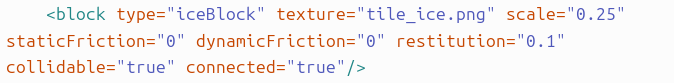
\includegraphics[width=1.0\textwidth]{images/XMLfile}
                \caption{Stockage d'un bloc au format XML}
            \end{figure}
        \column{0.4\textwidth}
            \begin{block}{Définition des blocs}
                \begin{itemize}
                    \item[\bullet] Définition des blocs au format XML
                    \item[\bullet] Lecture du fichier et stockage dans une classe dédiée
                    \item[\bullet] Accès depuis les autre classes via une méthode statique
                \end{itemize}
            \end{block}
    \end{columns}
\end{frame}

\begin{frame}{Connectivité des textures}
    \begin{columns}
        \column{0.4\textwidth}
            \begin{block}{Textures connectées}
                \begin{itemize}
                    \item[\bullet] Textures des blocs connectées aux blocs du même type
                    \item[\bullet] élément \emph{connected} du fichier XML
                    \item[\bullet] Textures au format de feuilles de sprite
                    \item[\bullet] Calcul basé sur les blocs autour
                \end{itemize}
            \end{block}
        \column{0.6\textwidth}
            \begin{figure}
                \centering
                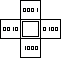
\includegraphics[width=0.8\textwidth]{images/connected_textures_offset_computing}
                \caption{Calcul de la texture connectée du bloc}
            \end{figure}
    \end{columns}
\end{frame}

\section{Présentation du personnage}
\begin{frame}{Contrôles de base}
    \begin{columns}
        \column{0.4\textwidth}
            \begin{block}{Contrôles du personnage}
                \begin{itemize}
                    \item[\bullet] Touches \emph{D} et \emph{Q}
                    \item[\bullet] Touches $\rightarrow$ et $\leftarrow$
                    \item[\bullet] Priorité à la direction droite
                    \item[\bullet] Dirigent le personnage
                \end{itemize}
            \end{block}
        \column{0.6\textwidth}
            \begin{figure}
                \centering
                
\includegraphics[width=0.8\textwidth]{images/character_placeholder.png}
                \caption{Personnage du jeu}
            \end{figure}
    \end{columns}
\end{frame}

\begin{frame}{Saut}
    \begin{block}{Saut}
        \begin{itemize}
            \item[\bullet] Touche \emph{Espace}
            \item[\bullet] Donne une impulsion vers le haut instantanée
            \item[\bullet] Permet de franchir des obstacles facilement
            \item[\bullet] Disponible depuis le sol
        \end{itemize}
    \end{block}
    \begin{block}{Double saut}
        \begin{itemize}
            \item[\bullet] Touche \emph{Espace} en l'air
            \item[\bullet] Utilisable une fois par saut
            \item[\bullet] Se recharge en touchant le sol

        \end{itemize}
    \end{block}
\end{frame}

\begin{frame}{Dash}
    \begin{block}{Dash}
        \begin{itemize}
            \item[\bullet] Impulsion directionnelle instantanée
            \item[\bullet] Activé en appuyant deux fois sur une touche directionnelle
            \item[\bullet] Permet de se déplacer rapidement horizontalement
            \item[\bullet] Disponible une seule fois en l'air
            \item[\bullet] Dispose d'un temps de recharge
        \end{itemize}
    \end{block}
\end{frame}

\begin{frame}{Score et vies}
    \begin{columns}
        \column{0.4\textwidth}
            Affichés à tout moment en haut à gauche
            \begin{block}{Vies du personnage}
                \begin{itemize}
                    \item[\bullet] Diminuent en touchant un pique
                    \item[\bullet] Une fois à 0, la partie se termine
                \end{itemize}
            \end{block}
            \begin{block}{Score}
                \begin{itemize}
                    \item[\bullet] S'incrémente en touchant un écrou
                    \item[\bullet] Score final affiché sur l'écran de fin
                \end{itemize}
            \end{block}
        \column{0.6\textwidth}
            \begin{figure}
                \centering
                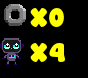
\includegraphics[width=0.8\textwidth]{images/Screenshot from 2025-03-23 23-14-37.png}
                \caption{Affichage du score et des vies}
            \end{figure}
    \end{columns}
\end{frame}

\section{La génération procédurale}
\begin{frame}{L'al\'eatoire}
    \begin{block}{Graine de génération}
        \begin{itemize}
            \item[\bullet] Choisie aléatoirement
            \item[\bullet] Peut être choisie manuellement
            \item[\bullet] Permet de reproduire les problèmes
        \end{itemize}
    \end{block}
\end{frame}

\begin{frame}{Génération des salles/des murs}
    \begin{columns}
        \column{0.5\textwidth}
        \begin{block}{Génération des salles}
            \begin{itemize}
                \item[\bullet] Génère une suite de salles connectées entre elles
                \item[\bullet] Éviter que les salles se chevauchent
                \item[\bullet] Retourne en arrière si aucun chemin n'est possible
            \end{itemize}
        \end{block}
        \column{0.4\textwidth}
        \begin{figure}
            \centering
            
\includegraphics[height=0.2\textheight]{images/room_placement}
            \caption{Placement d'une salle au dessus d'une autre}
        \end{figure}
        \begin{figure}
            \centering
            
\includegraphics[height=0.2\textheight]{images/filling_the_world}
            \caption{Génération des murs}
        \end{figure}
    \end{columns}
\end{frame}

\begin{frame}{Génération du chemin}
    \begin{columns}
        \column{0.5\textwidth}
        \begin{block}{Génération d'un chemin}
            \begin{itemize}
                \item[\bullet] Génère un chemin du début à la fin
                \item[\bullet] S'assurer que le niveau est possible
            \end{itemize}
        \end{block}
        \column{0.4\textwidth}
        \begin{figure}
            \centering
            
\includegraphics[width=1.0\textwidth]{images/two_ways_to_connect}
            \caption{Deux moyens de relier deux points du chemin}
        \end{figure}
    \end{columns}
\end{frame}

\begin{frame}{Les fausses platformes}
    \begin{columns}
        \column{0.5\textwidth}
        \begin{block}{Pourquoi?}
            \begin{itemize}
                \item[\bullet] Cache le vrai chemin
                \item[\bullet] Exploration du niveau
            \end{itemize}
        \end{block}
        \column{0.4\textwidth}
        \begin{figure}
            \centering
            
\includegraphics[width=1.0\textwidth]{images/fake_platforms}
            \caption{Une salle contenant de fausses plateformes}
        \end{figure}
    \end{columns}
\end{frame}

\begin{frame}{Les blocs spéciaux}
    \begin{columns}
        \column{0.5\textwidth}
        \begin{block}{Blocs de glace et de slime}
            \begin{itemize}
                \item[\bullet] Ajoute de la variété
                \item[\bullet] Généré à partir d'un bruit de Perlin
            \end{itemize}
        \end{block}
        \column{0.4\textwidth}
        \begin{figure}
            \centering
            
\includegraphics[height=0.2\textheight]{images/perlin_noise_example}
            \caption{Données brutes d'un bruit de Perlin}
        \end{figure}
        \begin{figure}
            \centering
            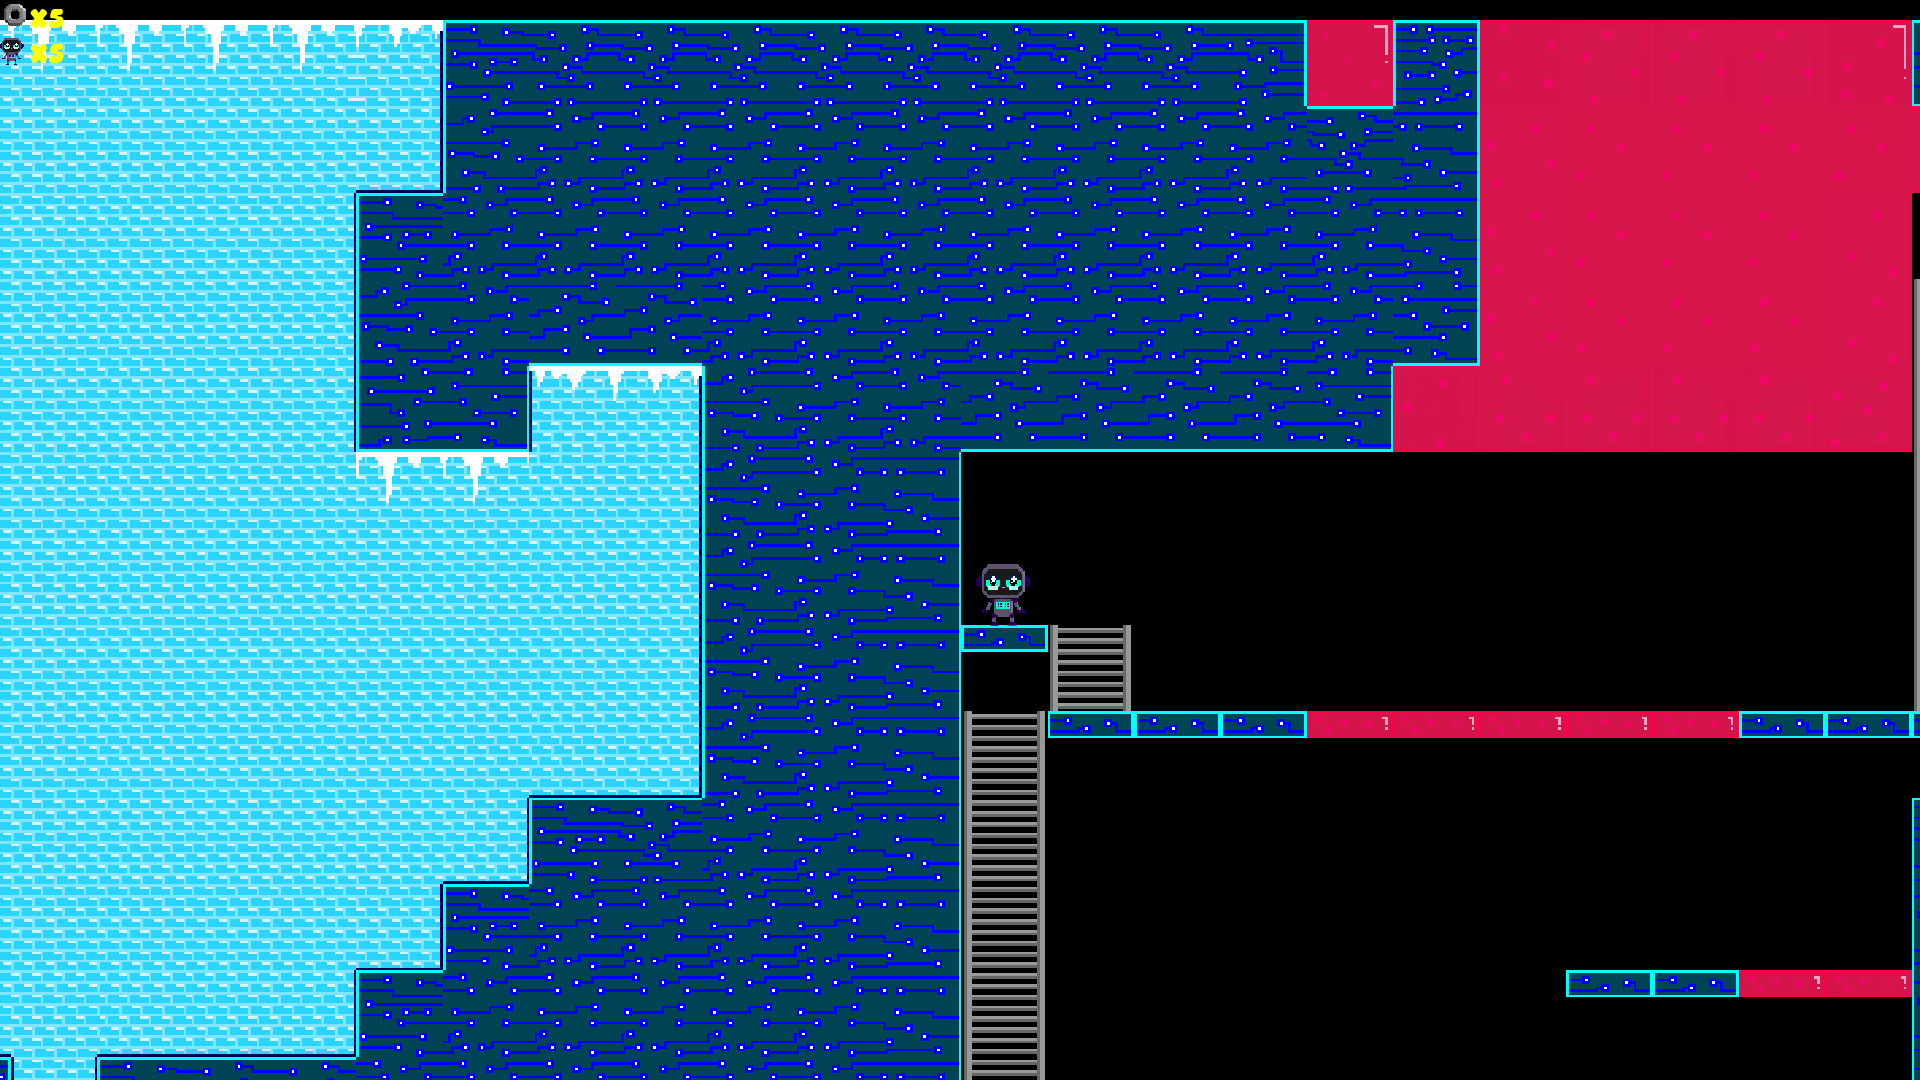
\includegraphics[height=0.2\textheight]{images/perlin_noise_in_level}
            \caption{Des blocs de glace et de slime dans un niveau}
        \end{figure}
    \end{columns}
\end{frame}

\begin{frame}{Les pièges}
    \begin{columns}
        \column{0.5\textwidth}
        \begin{block}{Génération de pics}
            \begin{itemize}
                \item[\bullet] Dans les salles dangereuses
                \item[\bullet] Au bout de lignes de blocs de glace
            \end{itemize}
        \end{block}
    \column{0.4\textwidth}
        \begin{figure}
            \centering
            
\includegraphics[width=1.0\textwidth]{images/ice_spike_trap}
            \caption{Deux situations où des pics peuvent se générer}
        \end{figure}
    \end{columns}
\end{frame}

\begin{frame}{Point d'apparition}
    \begin{columns}
        \column{0.5\textwidth}
        \begin{block}{Point d'apparition du joueur}
            \begin{itemize}
                \item[\bullet] Début du niveau
                \item[\bullet] Dans un endroit sûr
            \end{itemize}
        \end{block}
        \column{0.4\textwidth}
        \begin{figure}
            \centering
            
\includegraphics[width=1.0\textwidth]{images/valid_spawn_locations}
            \caption{Points d'apparition valides dans un niveau}
        \end{figure}
    \end{columns}
\end{frame}

\begin{frame}{Monde de test}
    \begin{columns}
        \column{0.5\textwidth}
        \begin{block}{Générateur de monde de test}
            \begin{itemize}
                \item[\bullet] Implémentation alternative d'un générateur de monde
                \item[\bullet] Permet de tester les fonctionnalités
            \end{itemize}
        \end{block}
        \column{0.4\textwidth}
        \begin{figure}
            \centering
            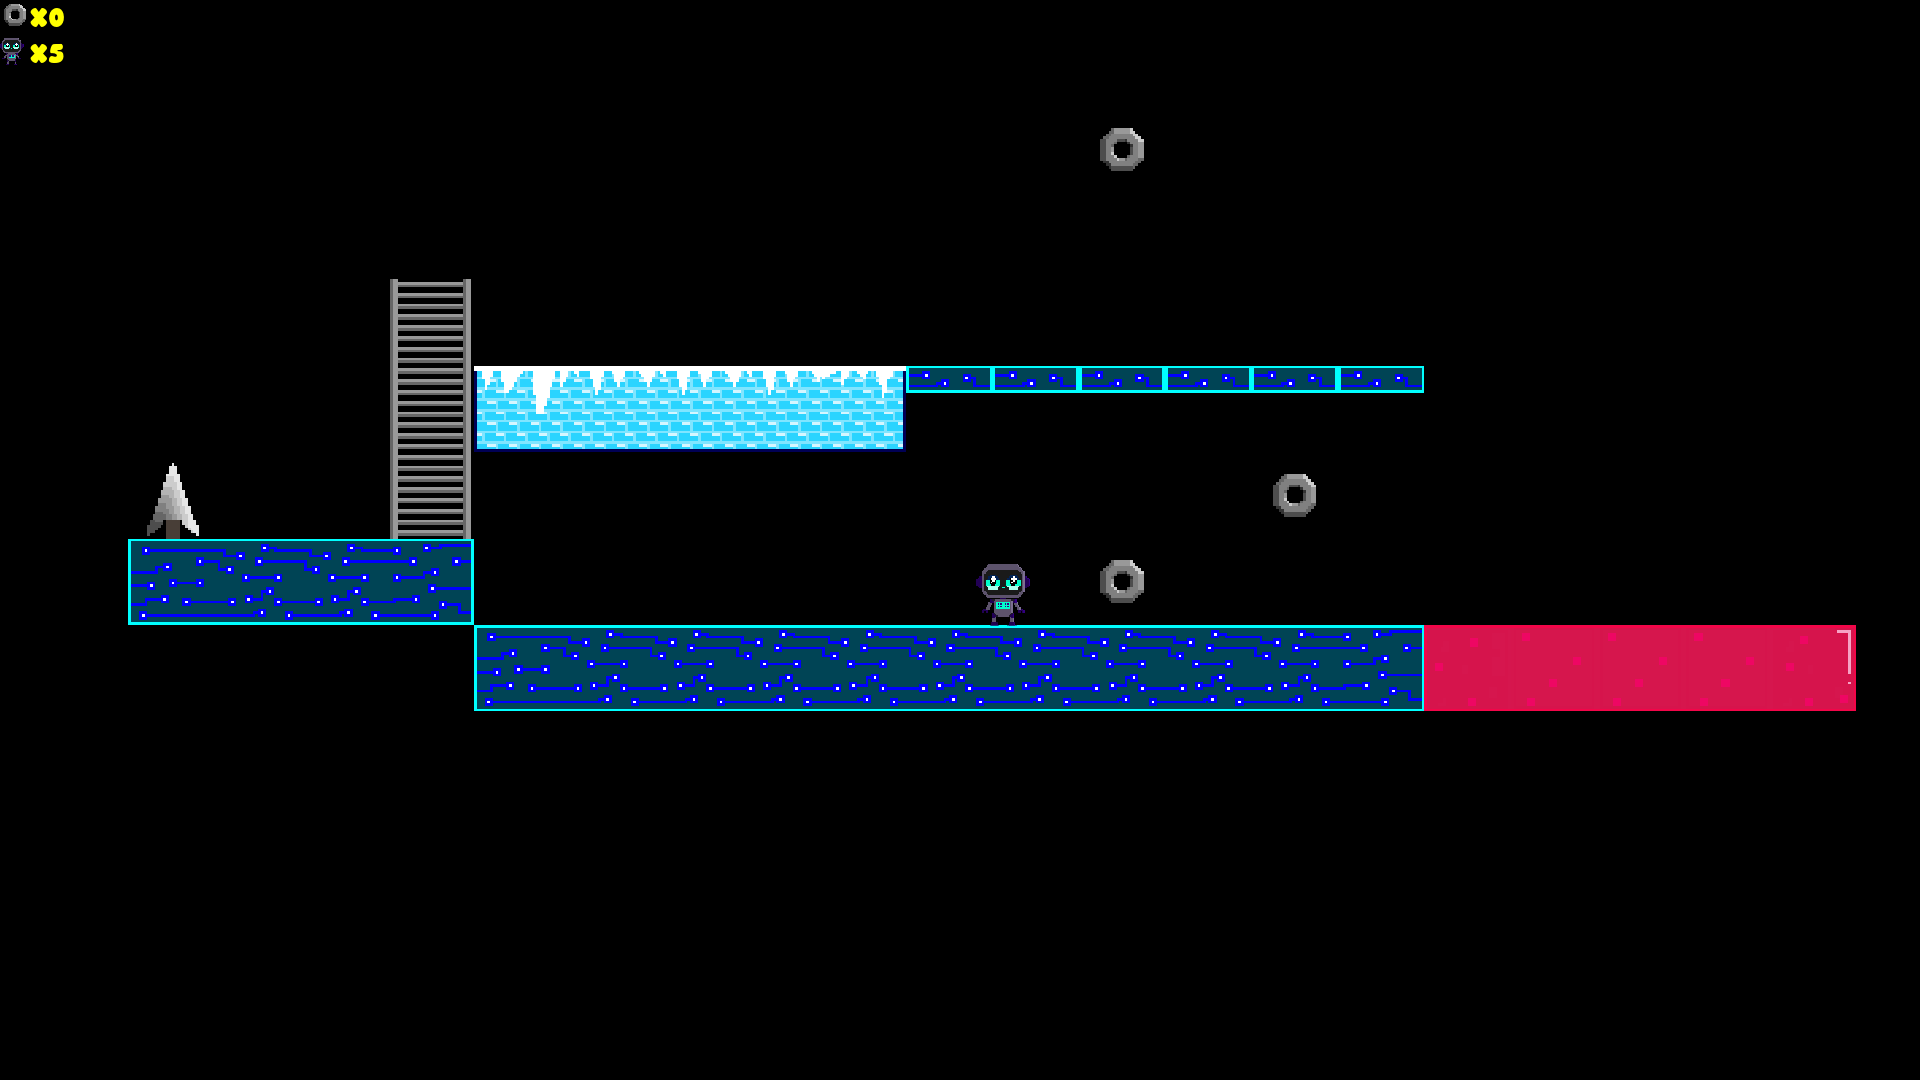
\includegraphics[width=1.0\textwidth]{images/test_world}
            \caption{Capture d'écran du monde de test}
        \end{figure}
    \end{columns}
\end{frame}

\section{La physique}
\begin{frame}{Gestion des collisions}
    Calcul de la vitesse relative de la collision :
    \[ V_{rel} =  - V_{joueur} \]
    Calcul de la vitesse par rapport à la normale :
    \[ V_{n} = V_{rel} \cdot n \]
    Calcul de la magnitude de l'impulsion à appliquer :
    \[ C_{i} = (1 + e) \times V_{n} \]
    Calcul du vecteur résultat :
    \[V_{res} = C_{i} \times n \]
    Application d'une correction (pour les erreurs de flottant) :
    \[V_{corr} = -max(d-0.1,0) \times C_{corr} \times n\]
\end{frame}

\begin{frame}{Platformes directionnelles}
    \begin{columns}
        \column{0.4\textwidth}
            \begin{block}{Platformes directionnelles}
                \begin{itemize}
                    \item[•] Utilisent une hitbox plus petite, dirigée
                    \item[•] élément \emph{direction} du fichier XML
                    \item[•] Le joueur utilise aussi une hitbox plus petite
                \end{itemize}
            \end{block}
        \column{0.6\textwidth}
            \begin{figure}
                \centering
                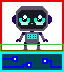
\includegraphics[width=0.5\textwidth]{images/DirectionnalHB.png}
                \caption{Hitbox directionnelle (en vert) comparée à la hitbox classique (en rouge)}
            \end{figure}
    \end{columns}
\end{frame}

\begin{frame}{Friction}
    Calcul de la tangente à la collision :
    \[t = V_{rel} - [V_{rel} \cdot (n \times (1,0))] \times n\]
    Calcul du coefficient de friction à appliquer :
    \[C_{f} = - V_{rel} \cdot t\]
    Calcul du vecteur de friction résultant :
    \[
        V_{friction} = \left\{\begin{array}{lr}
            C_{f} \times t & \text{si } |C_{f}| < |C_{i}| \times \mu_{s}\\
            -C_{i} \times t \times \mu_{d} & \text{si } |C_{f}| \geq |C_{i}| \times \mu_{s}
        \end{array}\right\}
    \]
\end{frame}

\begin{frame}{Autre données de physique}
    \begin{block}{Résistance de l'air}
        La résistance de l'air est donnée par :
        \[
         -dir \times (V_{joueur})^2 \times C_{air}
        \]
        avec \(C_{air} = (0.01,0.02)\)
    \end{block}

    \begin{block}{Collisions multiples}
        Moyenne des résultats des collisions avec les blocs
    \end{block}
\end{frame}

\section{Notre organisation}
\begin{frame}{Organisation du travail}

\end{frame}

\begin{frame}{Outils utilisés}

\end{frame}

\section{Conclusion}
\begin{frame}{Conclusion}

\end{frame}

\begin{frame}{Ce qu'on aurait voulu ajouter}
    \begin{block}{Elements d'amélioration}
        \begin{itemize}
          \item[\bullet] Des ennemis
          \item[\bullet] Des bulles
          \item[\bullet] Possibilité de choix de la graine de génération
          \item[\bullet] Clés
          \item[\bullet] Téléporteurs
          \item[\bullet] Des bonus
          \item[\bullet] Pluie/Eau
          \item[\bullet] Choix de difficulté
          \item[\bullet] Autre personnages
        \end{itemize}
    \end{block}
\end{frame}

\begin{frame}{Wave function collapse}
    \begin{columns}
        \column{0.5\textwidth}
        \begin{block}{Algorithme Wave Function Collapse}
            \begin{itemize}
                \item[\bullet] Arrange un ensemble de patternes donnés
                \item[\bullet] Pourrait être utilisé avec des morceaux de niveau
            \end{itemize}
        \end{block}
        \column{0.4\textwidth}
        \begin{figure}
            \centering
            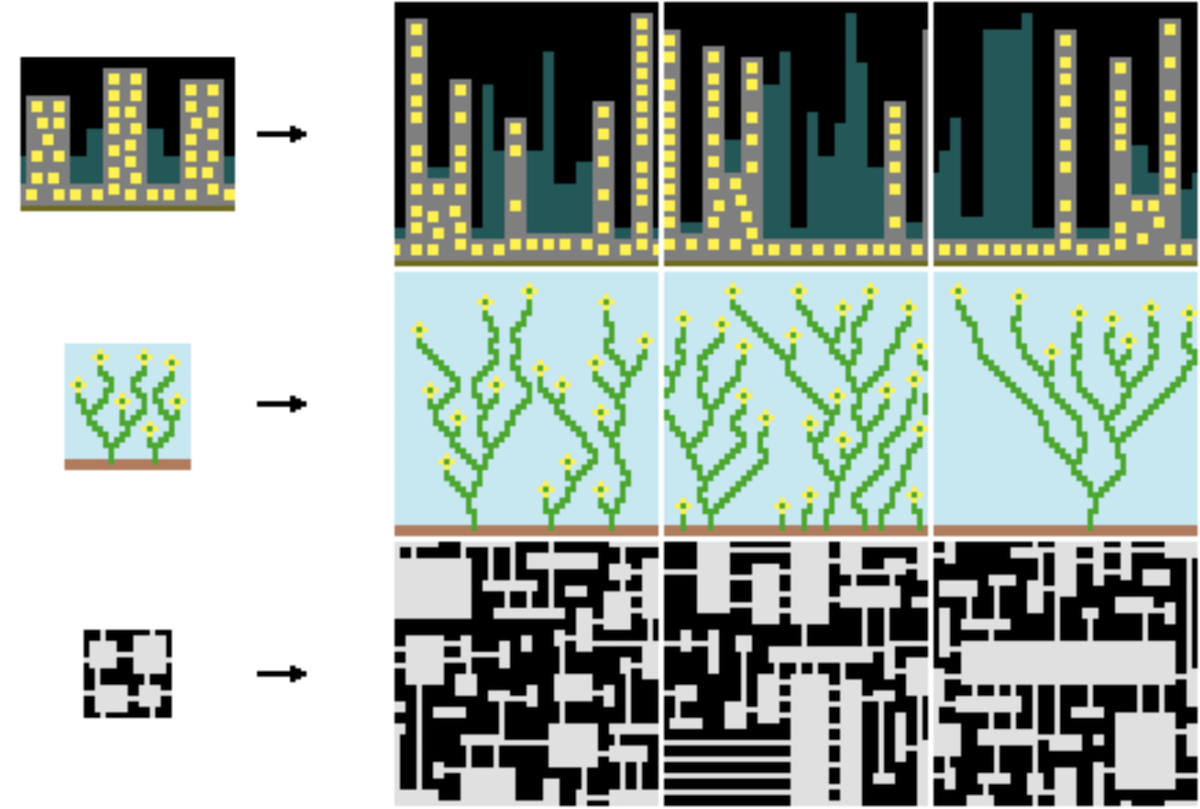
\includegraphics[width=1.0\textwidth]{images/wfc-examples}
            \caption{Des exemples d'application du Wave Function Collapse}
        \end{figure}
    \end{columns}
\end{frame}

\begin{frame}{Amélioration du pathfinding}
    \begin{block}{Meilleur pathfinding}
        \begin{itemize}
            \item[\bullet] Véritable algorithme de pathfinding
            \item[\bullet] Fonctionne 100\% du temps
            \item[\bullet] Prend en compte les contraintes
            \item[\bullet] Trajectoire rectiligne
        \end{itemize}
    \end{block}
\end{frame}

}

\begin{frame}[allowpagebreak,T]{Merci de nous avoir écouté}
    \centering
    Avez vous des questions ?
    \begin{figure}
        \centering
        
\includegraphics[width=0.5\linewidth]{images/character_placeholder.png}
    \end{figure}
\end{frame}

\end{document}
